\documentclass{ltjsarticle}
\usepackage[no-math]{fontspec} % 欧文フォント設定(和文フォント設定より先に行う)
\setmonofont[AutoFakeSlant,BoldItalicFeatures={FakeSlant}]{Inconsolatazi4} % Inoconsolataフォントを使用
\usepackage{upquote}
\usepackage[ipaex]{luatexja-preset} % 和文フォントにIPAexフォントを指定する
\usepackage{luatexja-adjust} % 行長調整
\usepackage{graphicx}
\usepackage[table]{xcolor}
%\usepackage{tabularx} % 表の全体幅が決まっている場合
%\usepackage{longtable} % ページをまたぐ表
%\usepackage{luatexja-ruby} % ルビ
\usepackage{tikz}
\usepackage[framemethod=tikz]{mdframed} % 枠で囲む
\usepackage{hyperxmp} % XMP support with hyperref
\usepackage[pdfencoding=auto,pdfa]{hyperref} % PDF/A compatible

%% 参考文献
\usepackage[backend=biber,style=numeric]{biblatex}
\addbibresource{refer.bib}

%% その他
\pdfminorversion=4 % PDF minor version (0-9)
\pdfcompresslevel=9 % PDF compress level (0 or 1-9)
\ltjenableadjust % JIS X 4051 互換の行長調整を行う
\renewcommand{\emph}[1]{\textsf{\textgt{#1}}} % 強調をゴシック体と Sans Serif に変更する

%% Kindle 用の設定 %%
%\setmainjfont[BoldFont=IPAexGothic]{KBMinchoM} % メインのフォントを KB明朝M に変更
%\usepackage[paperwidth=13.5cm, paperheight=17.25cm, top=0.5cm, left=0.5cm, right=0.5cm, bottom=0.5cm]{geometry} % Kindle layout

%% 文書情報
\title{\emph{クリエイティブ・コモンズ・ライセンスについて}}
\author{Spiegel}
\date{2014-09-11}

\hypersetup{% hyperref options (and metadata)
    pdflang={jp},
    pdftitle={クリエイティブ・コモンズ・ライセンスについて},
    pdfsubject={クリエイティブ・コモンズ・ライセンスについて日本の著作権法との関連を交えつつ解説していきたいと思います。},
    pdfauthor={Spiegel},
    pdfkeywords={Creative Commons, License, Copyright},
    pdfcopyright={Written by Spiegel on 2014, and licensed under CC-BY.},
    pdflicenseurl={http://creativecommons.org/licenses/by/4.0/},
    pdfcontacturl={http://www.baldanders.info/},
    pdfcontactcity={Hiroshima},
    pdfcontactcountry={Japan},
    pdfcontactregion={JA},
    pdfcaptionwriter={Spiegel},
    baseurl={http://www.baldanders.info/spiegel/archive/cc-license/},
    draft=false,
    bookmarks=true,
    bookmarksnumbered=true,
    bookmarksopen=false,
    colorlinks=true,
    linkcolor=red,
    citecolor=green,
    filecolor=magenta,
    urlcolor=cyan
}

\begin{document}

\maketitle
\tableofcontents
\clearpage

\section{クリエイティブ・コモンズ・ライセンスについて}

ここでは,クリエイティブ・コモンズ・ライセンス(以降cc-license)について日本の著作権法との関連を交えつつ解説していきます。

\subsection{cc-licenseは非排他的なライセンス(許可)を与えます}

cc-licenseは大雑把に言って「条件(requests)」と「許可(permissions)」で構成されています。
cc-licenseの条件には表\ref{tbl:cc-req}\footnote{\url{http://creativecommons.jp/licenses/}} の4つがあり,これらの条件を組み合わせて使います。
\begin{table}[htp]
\centering
\begin{tabular}{|>{\columncolor[gray]{0.8}}m{3.5cm}|>{\columncolor[gray]{0.8}}l|m{6cm}|}
    \hline
    
\includegraphics[width=1truecm,clip]{images/icons/by.pdf}    & \textgt{表示}     & 作品のクレジットを表示すること \\
    \hline
    
\includegraphics[width=1truecm,clip]{images/icons/nc.pdf}
    
\includegraphics[width=1truecm,clip]{images/icons/nc-eu.pdf}
    
\includegraphics[width=1truecm,clip]{images/icons/nc-jp.pdf} & \textgt{非営利}   & 営利目的での利用をしないこと \\
    \hline
    
\includegraphics[width=1truecm,clip]{images/icons/nd.pdf}    & \textgt{改変禁止} & 元の作品を改変しないこと \\
    \hline
    
\includegraphics[width=1truecm,clip]{images/icons/sa.pdf}    & \textgt{継承}     & 元の作品と同じ組み合わせのcc-licenseで公開すること \\
    \hline
\end{tabular}
\caption{cc-licenseの条件}\label{tbl:cc-req}
\end{table}%
ただし,「表示」は必須条件となっており,「改変禁止」と「継承」は条件が衝突するため同時に指定できません。
結局,表\ref{tbl:cc-req2}\,の6つの組み合わせが有効となっています\footnote{ロゴやアイコンの使用については\url{http://creativecommons.jp/policies/}\,を参照してください。}。
\begin{table}[htp]
\centering
\begin{tabular}{|>{\columncolor[gray]{0.8}}m{3.5cm}|l|}
    \hline
    
\includegraphics[width=2truecm,clip]{images/by.pdf}
    
\includegraphics[width=1.3truecm,clip]{images/by-s.pdf} & 表示 \\
    \hline
    
\includegraphics[width=2truecm,clip]{images/by-nc.pdf}
    
\includegraphics[width=1.3truecm,clip]{images/by-nc-s.pdf} & 表示-非営利 \\
    \hline
    
\includegraphics[width=2truecm,clip]{images/by-sa.pdf}
    
\includegraphics[width=1.3truecm,clip]{images/by-sa-s.pdf} & 表示-継承 \\
    \hline
    
\includegraphics[width=2truecm,clip]{images/by-nc-sa.pdf}
    
\includegraphics[width=1.3truecm,clip]{images/by-nc-sa-s.pdf} & 表示-非営利-継承 \\
    \hline
    
\includegraphics[width=2truecm,clip]{images/by-nd.pdf}
    
\includegraphics[width=1.3truecm,clip]{images/by-nd-s.pdf} & 表示-改変禁止 \\
    \hline
    
\includegraphics[width=2truecm,clip]{images/by-nc-nd.pdf}
    
\includegraphics[width=1.3truecm,clip]{images/by-nc-nd-s.pdf} & 表示-非営利-改変禁止 \\
    \hline
\end{tabular}
\caption{cc-license条件の組み合わせ}\label{tbl:cc-req2}
\end{table}%
これらの条件(の組み合わせ)を守る限り,ライセンスを受けるユーザ(licensee)は以下に示す非排他的(または非独占的)な「利用」が可能です。
\begin{itemize}
\item 作品をコピーすること
\item コピーした作品を配布すること
\item コピーした作品を公の場で展示・演奏すること
\item コピーした作品をデジタル形式によって公の場で展示・演奏すること
\item 作品を同一状態で別の形式に変換すること(逐語的コピー)
\item 作品を改変し公表すること(二次的著作物,ただし改変禁止の条件がない場合)
\end{itemize}
二次的著作物の例としては編集,編曲,翻訳,脚色,パロディ化,データベース化といったものが挙げられます(二次的著作物については\ref{sec:adaptations}節で更に詳しく紹介します)。
また,以下の「利用」については条件によらずlicenseeには許可されていません。
\begin{itemize}
\item 作品およびそのコピーについて,著作権表示を改変・削除すること
\item 作品およびそのコピーについて,ライセンスおよびその条件を変更すること
\item 作品の正当な「使用」または許可された「利用」を制限する技術的保護手段を用いること(技術的保護手段については\ref{sec:drm}節で更に詳しく紹介します)
\end{itemize}
さらに,licenseeがcc-licenseによって定めた条件(営利目的利用,二次的著作物など)を超える利用を行いたい場合は,licensorである著作(権)者から個別に許可を得る必要があります。
(たとえば,自分の作品にcc-licenseを付与しつつロイヤリティを得たい場合は,cc-licenseに「非営利」の条件を付け,営利目的で利用したいユーザ向けには個別に契約を行う,といった方法もあります)


\subsection{cc-licenseは法的拘束力を持つ「契約」です}

cc-licenseについてよくある誤解は「cc-licenseは法的拘束力のないガイドラインである」というものですが,実際にはcc-licenseは法的拘束力を持つ「契約」です(したがってlicensorである著作(権)者はcc-licenseによって一度定めた許可を取り消すことはできません)。
cc-licenseは以下の3つのレイヤで構成されています。
\begin{quote}\begin{description}
\item[コモンズ証(Commons Deed)] :\par
    cc-licenseの条件と許可についてHuman-Readableな形で記述したもの。
\item[法的条項(Legal Code)] :\par
    c-licenseの内容をLawyer-Readableな形で記述した「利用許諾書」。
    法的条項によってcc-licenseが法的拘束力を持つことを担保する。
\item[メタデータ(Metadata)] :\par
    作品に関する(著作権・ライセンスを含む)情報をMachine-Readableな形で記述したもの。
    記述形式としてはRDFa, XMPなどがあるが,Web上ではRDFaがよく用いられる。
    メタデータはGoogleなどの検索エンジンでparseされ,ネット上の数多の作品を利用条件によって検索可能とする。
\end{description}\end{quote}

日本の作品(著作物)の場合cc-licenseは日本の著作権法を準拠法とします。
また日本の著作権法はベルヌ条約をはじめとする国際的な取り決めの中で運用されています。
したがってcc-licenseは
\begin{itemize}
\item 世界中で適用されます。
\item 作品の著作権の存続期間の間,持続します。
\end{itemize}
さらにクリエイティブ・コモンズやcc-licenseはlicensorである著作(権)者から権利を奪いません(言い方を変えれば作品は著作(権)者自身が管理する必要があります)。
またクリエイティブ・コモンズやcc-licenseはユーザであるlicenseeに対して,fair use(公正な利用),firstsale doctrine(最初の頒布(取引)で権利が消尽すること),表現の自由等の権利を侵害することもありません。


\subsection{cc-licenseは作品の「使用」を制限しません} \label{sec:fair use}

著作権は,著作(権)者が明示的に許可しない限り,作品(著作物)の「利用」を制限できます。
利用として挙げられるものは以下のとおりです。
\begin{itemize}
\item 複製(一部または全部,デジタル化を含む),上演,演奏,上映,公衆送信,口述,展示,頒布,譲渡,貸与
\item 二次的著作物(\ref{sec:adaptations}節)の作成・複製・頒布・譲渡
\item 編集,データベース化
\end{itemize}

一方で,例えば書籍を読んだり音楽を聴いたり建築物に住んだりプログラムを実行したり,といった行為は作品(著作物)の「使用」とみなされ制限の範囲外となります。
たとえば,ある作品の海賊版(著作(権)者によって許可されない利用)が出回っている場合,(海賊版の出版は著作権に触れますが)海賊版を見たり聞いたりする行為は「使用」なので著作権は関知しません。
あるいは作品の利用や使用の前段階としての「作品へのアクセス」も著作権の範囲外です\footnote{とはいえ,実際には作品の「使用」と「利用」の境界は曖昧で,時にこれが議論になります。実はcc-licenseにはこうした曖昧さを「条件」と「許可」を明示的に設定することで回避する狙いもあります。}。

また作品の利用の一部については「権利の制限」として著作(権)者の許可無く(無断で)行うことができます。
「権利の制限」の対象となる利用については以下のものがあります。
\begin{itemize}
\item 私的複製
      \begin{itemize}
      \item 個人のみが対象,企業のような営利目的を持った団体は含まれない
      \item 複製する者の属するグループのメンバー相互間に強い個人的結合関係のあることが必要(実質的には家族や親しい友人グループ間のみ)
      \item コピー機のような自動複製機器を公衆の場に置いて利用する場合は私的複製として認められない場合がある
      \item 技術的保護手段の回避は私的複製として認められない(DVD の暗号化を解除してリッピングするなど)
      \end{itemize}
\item 図書館等における複製
      \begin{itemize}
      \item 利用者の求めに応じてその調査研究用に複製物を提供する場合
            \begin{itemize}
            \item 資料の一部(少なくとも半分以下)のみが対象
            \item 発行後相当期間が経過した雑誌等に掲載された個々の著作物(記事・論文など)は全部複製することが可能
            \item 営利を目的としないこと
            \end{itemize}
      \item 図書館資料の保存上必要な場合
      \item 他の図書館等の求めに応じて入手困難な資料の複製物を提供する場合
      \item 国立国会図書館では絶版の著作物のデジタル複製と\emph{自動公衆送信}が可能
      \item 国立国会図書館法によるインターネット資料の複製
      \end{itemize}
\item 引用
      \begin{itemize}
      \item 引用の対象となる作品が公表されていること
      \item 公正な慣行に合致していること(「批判」のための引用は公正な慣行です)
      \item 引用の目的上正当な範囲であること
      \item 引用部分が識別できること
      \item 引用されて利用される側の著作物の出所を明記すること
      \item 自分の作品が主で,引用される部分が従になっていること
      \end{itemize}
\item 視聴覚障害者のための複製
      \begin{itemize}
      \item 公表された著作物を視覚障害者向けの点字にして複製することが可能
      \item 視覚障害者向けの貸し出し用に公表された著作物を録音することが可能
      \item 放送中の番組に限ってインターネットで字幕を流すことが可能
      \end{itemize}
\item 教育目的の複製
      \begin{itemize}
      \item 教科書への掲載
      \item 学校教育番組の放送
      \item 教育機関(学校など)で著作物のコピーをする時
            \begin{itemize}
            \item 継続的ではない講習会,個人経営で営利を目的としている塾や予備校などは含まれない
            \item 複製は授業に用いるためでなくてはならず,複製する人はその授業をする人でなければならない
            \item 複製の範囲は,授業のために必要と認められる限度の量で枚数は出席する学生の数まで
            \end{itemize}
      \item 試験問題として複製
      \item 視覚障害・発達障害等の児童・生徒のために教科書の内容を複製し拡大教科書を作成できる(非営利のみ)
      \end{itemize}
\item 営利を目的としない利用
      \begin{itemize}
      \item 上演権・演奏権・上映権・口述権・有線放送権・伝達権・貸与権が対象(映画の著作物は除く)
      \item 営利を目的とせず,聴衆や観衆などから料金を受けていない場合
      \end{itemize}
\item 付随的利用
      \begin{itemize}
      \item 写真の撮影、録音又は録画の方法によつて著作物を創作する場合
      \item 分離することが困難であるため付随して対象となる事物又は音に係る他の著作物(付随対象著作物)が対象
      \item 付随対象著作物の複製,翻案が可能で,付随対象著作物を含む作品を著作(権)者の許可に従って利用することが可能
      \item 著作権者の利益を不当に害する場合は利用できない
      \end{itemize}
\item 時事問題に関する論説の転載等
\item 政治上の演説などの利用
\item 裁判手続き等における複製
\item 行政機関情報公開法などによる開示のための利用
\item 公開の美術の著作物等の利用
\item 美術の著作物等の展示に伴う複製
\item 検討の過程における利用
\item 技術の開発又は実用化のための試験に用いるための利用
\item インターネット・オークション等の商品紹介用画像の掲載のための複製
\item プログラムの所有者による複製など
\item 保守・修理のための一時的複製
\item 送信障害の防止等のための複製(ミラーリング・バックアップ・キャッシング等)
\item インターネット情報検索サービスにおける複製
\item 情報解析のための複製
\item コンピュータにおける著作物利用に伴う複製
\item インターネットサービスの準備に伴う記録媒体への記録・翻案
\item 複製物の制限により作成された複製物の譲渡
\end{itemize}

cc-licenseでは作品の「使用」および「権利の制限」として認められている「利用」について制限しません。


\subsection{cc-license のバージョン}

現在,cc-licenseとして日本で有効なバージョンは以下のとおりです。
\begin{itemize}
\item バージョン1.0 Generic
\item バージョン2.0 Generic
\item バージョン2.1 日本版
\item バージョン2.5 Generic
\item バージョン3.0 Unported
\item バージョン4.0 International
\end{itemize}
このうち,厳密に日本法を準拠法として明記し,かつ法的に日本に最適化されているバージョンは「バージョン2.1日本版」のみです(表\ref{tbl:cc-license-2.1jp})。
\begin{table}[htp]
\centering
\begin{tabular}{|>{\columncolor[gray]{0.8}}m{3.5cm}|>{\columncolor[gray]{0.8}}l|m{4cm}|}
    \hline
    
\includegraphics[width=2truecm,clip]{images/by.pdf}
    
\includegraphics[width=1.3truecm,clip]{images/by-s.pdf} &
    表示 &
    \href{http://creativecommons.org/licenses/by/2.1/jp/}{コモンズ証},
    \href{http://creativecommons.org/licenses/by/2.1/jp/legalcode}{法的条項},
    \href{http://creativecommons.org/licenses/by/2.1/jp/rdf}{メタデータ}
    \\
    \hline
    
\includegraphics[width=2truecm,clip]{images/by-nc.pdf}
    
\includegraphics[width=1.3truecm,clip]{images/by-nc-s.pdf} &
    表示-非営利 &
    \href{http://creativecommons.org/licenses/by-nc/2.1/jp/}{コモンズ証},
    \href{http://creativecommons.org/licenses/by-nc/2.1/jp/legalcode}{法的条項},
    \href{http://creativecommons.org/licenses/by-nc/2.1/jp/rdf}{メタデータ}
    \\
    \hline
    
\includegraphics[width=2truecm,clip]{images/by-sa.pdf}
    
\includegraphics[width=1.3truecm,clip]{images/by-sa-s.pdf} &
    表示-継承 &
    \href{http://creativecommons.org/licenses/by-sa/2.1/jp/}{コモンズ証},
    \href{http://creativecommons.org/licenses/by-sa/2.1/jp/legalcode}{法的条項},
    \href{http://creativecommons.org/licenses/by-sa/2.1/jp/rdf}{メタデータ}
    \\
    \hline
    
\includegraphics[width=2truecm,clip]{images/by-nc-sa.pdf}
    
\includegraphics[width=1.3truecm,clip]{images/by-nc-sa-s.pdf} &
    表示-非営利-継承 &
    \href{http://creativecommons.org/licenses/by-nc-sa/2.1/jp/}{コモンズ証},
    \href{http://creativecommons.org/licenses/by-nc-sa/2.1/jp/legalcode}{法的条項},
    \href{http://creativecommons.org/licenses/by-nc-sa/2.1/jp/rdf}{メタデータ}
    \\
    \hline
    
\includegraphics[width=2truecm,clip]{images/by-nd.pdf}
    
\includegraphics[width=1.3truecm,clip]{images/by-nd-s.pdf} &
    表示-改変禁止 &
    \href{http://creativecommons.org/licenses/by-nd/2.1/jp/}{コモンズ証},
    \href{http://creativecommons.org/licenses/by-nd/2.1/jp/legalcode}{法的条項},
    \href{http://creativecommons.org/licenses/by-nd/2.1/jp/rdf}{メタデータ}
    \\
    \hline
    
\includegraphics[width=2truecm,clip]{images/by-nc-nd.pdf}
    
\includegraphics[width=1.3truecm,clip]{images/by-nc-nd-s.pdf} &
    表示-非営利-改変禁止 &
    \href{http://creativecommons.org/licenses/by-nc-nd/2.1/jp/}{コモンズ証},
    \href{http://creativecommons.org/licenses/by-nc-nd/2.1/jp/legalcode}{法的条項},
    \href{http://creativecommons.org/licenses/by-nc-nd/2.1/jp/rdf}{メタデータ}
    \\
    \hline
\end{tabular}
\caption{cc-licenseバージョン2.1日本版}\label{tbl:cc-license-2.1jp}
\end{table}%
ただし,日本版以外のバージョンも日本発の作品であれば日本法を準拠法として解釈されるため通常は問題ありません\footnote{国際取引の場合はどの国を準拠法とするかで問題になる場合があります。これを避けるために著作権表記にあらかじめ管轄地を明記しておく方法もあります。}。

Generic / Unported / Internationalの各バージョンについては,可能であれば最新版(4.0 International,表\ref{tbl:cc-license-4.0})にアップデートすることを検討してみてください。
cc-licenseは常に議論され改良されています\footnote{\url{http://wiki.creativecommons.org/}}。
\begin{table}[htp]
\centering
\begin{tabular}{|>{\columncolor[gray]{0.8}}m{3.5cm}|>{\columncolor[gray]{0.8}}l|m{4cm}|}
    \hline
    
\includegraphics[width=2truecm,clip]{images/by.pdf}
    
\includegraphics[width=1.3truecm,clip]{images/by-s.pdf} &
    表示 &
    \href{http://creativecommons.org/licenses/by/4.0/}{コモンズ証}(\href{http://creativecommons.org/licenses/by/4.0/deed.ja}{日本語}),
    \href{http://creativecommons.org/licenses/by/4.0/legalcode}{法的条項},
    \href{http://creativecommons.org/licenses/by/4.0/rdf}{メタデータ}
    \\
    \hline
    
\includegraphics[width=2truecm,clip]{images/by-nc.pdf}
    
\includegraphics[width=1.3truecm,clip]{images/by-nc-s.pdf} &
    表示-非営利 &
    \href{http://creativecommons.org/licenses/by-nc/4.0/}{コモンズ証}(\href{http://creativecommons.org/licenses/by-nc/4.0/deed.ja}{日本語}),
    \href{http://creativecommons.org/licenses/by-nc/4.0/legalcode}{法的条項},
    \href{http://creativecommons.org/licenses/by-nc/4.0/rdf}{メタデータ}
    \\
    \hline
    
\includegraphics[width=2truecm,clip]{images/by-sa.pdf}
    
\includegraphics[width=1.3truecm,clip]{images/by-sa-s.pdf} &
    表示-継承 &
    \href{http://creativecommons.org/licenses/by-sa/4.0/}{コモンズ証}(\href{http://creativecommons.org/licenses/by-sa/4.0/deed.ja}{日本語}),
    \href{http://creativecommons.org/licenses/by-sa/4.0/legalcode}{法的条項},
    \href{http://creativecommons.org/licenses/by-sa/4.0/rdf}{メタデータ}
    \\
    \hline
    
\includegraphics[width=2truecm,clip]{images/by-nc-sa.pdf}
    
\includegraphics[width=1.3truecm,clip]{images/by-nc-sa-s.pdf} &
    表示-非営利-継承 &
    \href{http://creativecommons.org/licenses/by-nc-sa/4.0/}{コモンズ証}(\href{http://creativecommons.org/licenses/by-nc-sa/4.0/deed.ja}{日本語}),
    \href{http://creativecommons.org/licenses/by-nc-sa/4.0/legalcode}{法的条項},
    \href{http://creativecommons.org/licenses/by-nc-sa/4.0/rdf}{メタデータ}
    \\
    \hline
    
\includegraphics[width=2truecm,clip]{images/by-nd.pdf}
    
\includegraphics[width=1.3truecm,clip]{images/by-nd-s.pdf} &
    表示-改変禁止 &
    \href{http://creativecommons.org/licenses/by-nd/4.0/}{コモンズ証}(\href{http://creativecommons.org/licenses/by-nd/4.0/deed.ja}{日本語}),
    \href{http://creativecommons.org/licenses/by-nd/4.0/legalcode}{法的条項},
    \href{http://creativecommons.org/licenses/by-nd/4.0/rdf}{メタデータ}
    \\
    \hline
    
\includegraphics[width=2truecm,clip]{images/by-nc-nd.pdf}
    
\includegraphics[width=1.3truecm,clip]{images/by-nc-nd-s.pdf} &
    表示-非営利-改変禁止 &
    \href{http://creativecommons.org/licenses/by-nc-nd/4.0/}{コモンズ証}(\href{http://creativecommons.org/licenses/by-nc-nd/4.0/deed.ja}{日本語}),
    \href{http://creativecommons.org/licenses/by-nc-nd/4.0/legalcode}{法的条項},
    \href{http://creativecommons.org/licenses/by-nc-nd/4.0/rdf}{メタデータ}
    \\
    \hline
\end{tabular}
\caption{cc-licenseバージョン4.0 International}\label{tbl:cc-license-4.0}
\end{table}%


\subsection{cc-licenseのメタデータ} \label{sec:metadata}

cc-licenseではメタデータの記述にRDF(Resource Description Framework)\cite{Book:KANZAKI-RDF}\,を用います。
RDFの記述形式としてはXMLやRDFa\footnote{RDFaについては拙文「\href{http://www.baldanders.info/spiegel/archive/rdfa/}{RDFa入門}」を参照して下さい。(\cite{Book:KANZAKI-SHX}\,も参考になります)
} などが用いられますが,ここではRDF/XMLを用いたXMP(Extensible Metadata Platform)を紹介します。

XMPはPDFやExif(画像データ用のメタデータ規格)などにXML形式のデータをパケットとして埋め込むものです。
XMPは図\ref{fig:xmp}\,のように記述します。
\begin{figure}[htp]
\begin{mdframed}
\small
\begin{verbatim}
<?xpacket begin="<BOM>"id="W5M0MpCehiHzreSzNTczkc9d"?>
<x:xmpmeta xmlns:x="adobe:ns:meta/" x:xmptk="3.1-702">
  <rdf:RDF xmlns:rdf="http://www.w3.org/1999/02/22-rdf-syntax-ns#">
    [...]
  </rdf:RDF>
</x:xmpmeta>
<?xpacket end="w"?>
\end{verbatim}
\end{mdframed}
\caption{XMPパケット} \label{fig:xmp}
\end{figure}%
\verb|[...]|\,部分に実際の情報をRDF/XMLで記述します。
\verb|begin="<BOM>"|\,の部分にはUnicodeのBOM(byte order mark)をセットします。

ドキュメント組版システムである\TeX(pdf\LaTeX\,またはLua\LaTeX)を使ってPDFファイルを作成する場合は,hyperrefおよびhyperxmpパッケージを使ってXMPパケットを埋め込むことができます。
具体的には文書ファイルのプリアンブル部に図\ref{fig:hyperxmp}\,のように設定します。
\begin{figure}[htp]
\begin{mdframed}
\small
\begin{verbatim}
\usepackage{hyperxmp} % XMP support with hyperref
\usepackage[pdfencoding=auto]{hyperref}

\hypersetup{% hyperref options (and metadata)
    pdflang={jp},
    pdftitle={クリエイティブ・コモンズ・ライセンスについて},
    pdfsubject={クリエイティブ・コモンズ・ライセンスについて...},
    pdfauthor={Spiegel},
    pdfkeywords={Creative Commons, License, Copyright},
    pdfcopyright={Written by Spiegel on 2014, and licensed under CC-BY.},
    pdflicenseurl={http://creativecommons.org/licenses/by/4.0/},
    pdfcaptionwriter={Spiegel}
}
\end{verbatim}
\end{mdframed}
\caption{Lua\LaTeX\,によるメタデータの設定} \label{fig:hyperxmp}
\end{figure}%
この記述によってタイトル・著者名・著作権表記・ライセンスへのURLなどの情報をXMPパケットとして埋め込むことができます。
\verb|pdflicenseurl|\,でcc-licenseのコモンズ証へのURLが指定されているのがわかると思います。
この状態でタイプセットするとPDFに著作権情報が埋め込まれます(図\ref{fig:pdf-prop})\footnote{ただし,この方法でPDFを作成すると,どういうわけかAdobe Readerでは「タグ付きPDF」として認識されません。}。
\begin{figure}[htp]
\begin{center}
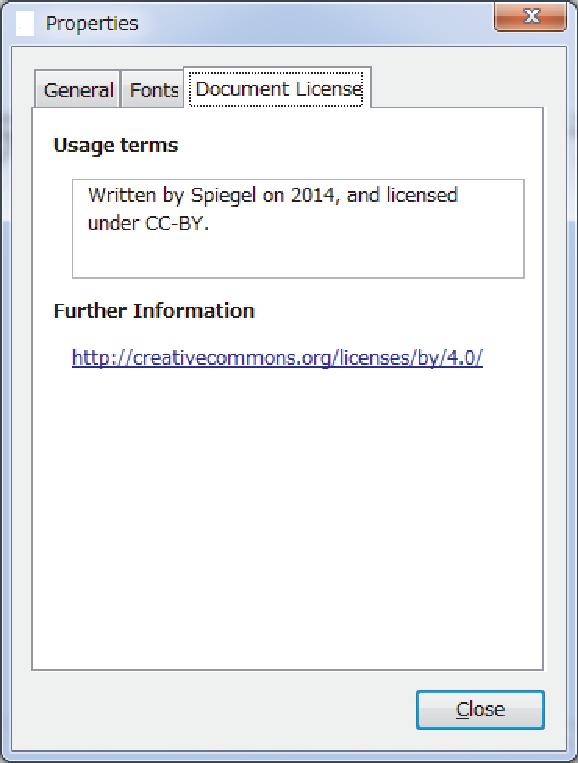
\includegraphics[width=5truecm,clip]{images/pdf-property.pdf}
\end{center}
\caption{PDFのプロパティ(\href{https://wiki.gnome.org/Apps/Evince}{Evince}\,で確認)} \label{fig:pdf-prop}
\end{figure}%

自身の作品について著作権表示をおこなう際に最低限必要なのは「著作(権)者名」と「作成日(または年)」です(著作(権)者名は本名でなくとも構いません)。
これにcc-licenseを加えた3点が正しく表示されているかどうか注意して下さい。

著作者であれば作品を作成した時点で自動的に権利が付与されますので ``Copyright \copyright'' は付けなくとも自明です\footnote{\copyright\,マークは著作権が登録制だった時代の名残です。現在はベルヌ条約に基づき著作権は自動的に著作者に付与されます。}。
ただし何らかの形で権利が譲渡されている(つまり著作者と著作権者が異なっている)場合は表記に注意が必要です。
もちろん(たとえ著作者であっても)権利のない人が勝手にライセンスを設定することはできません。

他者の作品を転載(複製・配布)したり二次的著作物の場合は,原則としてオリジナルの著作権情報を付記します\footnote{著作(権)者がこれを求めない場合もあります。cc-licenseでは著作(権)者であるlicensorが二次的著作物へのクレジット表記を削除するよう要請することができます。}。
オリジナル作品がcc-licenseの場合は
\begin{enumerate}
\item オリジナル作品の(権利の帰属先としての)著作(権)者名
\item オリジナル作品のライセンス表記(追加許諾があればそれも併せて)
\item オリジナル作品の免責事項等(もしあれば)
\item オリジナル作品を示す URI またはハイパーリンク(もしあれば)
\end{enumerate}
があることを確認して下さい。
ただしハイパーリンク先に最初の3つの表示があればハイパーリンクの明示だけでもOKです。


\section{雑多なこと}

\subsection{cc-licenseと人格権}

日本の著作権法には複製権や頒布権といった「著作財産権」の他に「著作者人格権」があります。
著作財産権は譲渡可能ですが,著作者人格権は譲渡や放棄はできませんし\footnote{著作者に対し著作者人格権の不行使を強制することもできません。} 著作者以外の人が行使することもできません。
著作者人格権は以下の権利で構成されています。
\begin{itemize}
\item 公表権
\item 氏名表示権
\item 同一性保持権
\end{itemize}
このうちもっとも強力な権利が「同一性保持権」です。
日本では(著作者の意に反しているかどうかに関わらず)作品の改変を著作者によって禁止することができます。
例外はいくつかありますが,このような強い権利は他の国にはありません\footnote{同一性保持権自体は他の国でも見られますが,かなり限定的です。}。
このため日本の著作権ライセンスの中にはlicensorによる「同一性保持権」の不行使を明示しているものもあります。

cc-license日本版では著作者人格権の行使に関しては限定的で
\begin{mdframed}
「原著作者及び実演家の名誉又は声望を害する方法で原著作物を改作、変形もしくは翻案して生じる著作物は、この利用許諾の目的においては、二次的著作物に含まれない」\par
(「\href{http://creativecommons.org/licenses/by-sa/2.1/jp/legalcode}{クリエイティブ・コモンズ リーガル・コード}」第1条aより)
\end{mdframed}
となっていて,結果的に著作者の名誉・声望を害する形での改変は許可されないことになっています(これ以外の人格権の行使は明示的に「行使しない」(第3条)となっています)。

cc-license 4.0 Internationalでは,著作者人格権はライセンスされない,とあります\footnote{パブリシティー権・プライバシー権といった人格権類似の権利についてもライセンスしないとあります。}。
\begin{mdframed}
 ``Moral rights, such as the right of integrity, are not licensed under this Public License, nor are publicity, privacy, and/or other similar personality rights; however, to the extent possible, the Licensor waives and/or agrees not to assert any such rights held by the Licensor to the limited extent necessary to allow You to exercise the Licensed Rights, but not otherwise.'' \par
(via  ``\href{http://creativecommons.org/licenses/by-sa/4.0/legalcode}{Creative Commons — Attribution-ShareAlike 4.0 International}''  Section 2 b1)
\end{mdframed}
ただし「可能な限り[...]権利を主張しない」ともあります。


\subsection{cc-licenseと著作隣接権}

日本の著作権法には更に「著作隣接権」が存在します。
「著作隣接権」は以下の権利で構成されています。
\begin{itemize}
\item 実演家(俳優・舞踏家・演奏家・歌手など)の権利
\item レコード製作者の権利
\item 放送事業者の権利
\item 有線放送事業者の権利
\end{itemize}
cc-license日本版では著作隣接権者についても配慮されています。
先の人格権についても「実演家の人格権」を含めた記述になっています。
また著作隣接権者をlicensorに含めるとなると厳密な意味での「著作物」を超える範囲を取り扱うことになります\footnote{著作権の存続期間の切れた古典芸能の実演や自然の鳥の声などを録音したレコードなど。}。
そこで日本版ではライセンスの目的物を「著作物」だけではなく,それらを含めた「作品」として取り扱えるようになっています。

cc-license 4.0 Internationalでは ``Similar Rights'' として隣接権にも配慮した記述になっています。


\subsection{二次的著作物の著作権} \label{sec:adaptations}

日本の著作権法では「二次的著作物」を以下のように定義しています。
\begin{itemize}
\item 翻訳
\item 編曲
\item 変形(翻訳・編曲以外で既存の著作物を他の表現形式で表現すること)
      \begin{itemize}
      \item 美術、写真、建築物、地図・図形の著作物で用いられる事が多い
            \begin{itemize}
            \item 写真を絵画にする
            \item 絵画を彫刻にする
            \end{itemize}
      \end{itemize}
\item 翻案(翻訳,編曲,変形以外のすべての改変をさす)
      \begin{itemize}
      \item 脚色,映画化・漫画化・小説化など
      \item プログラムのバージョンアップや他言語への移植なども翻案とみなされる
      \end{itemize}
\end{itemize}
ここでポイントとなるのは,二次的著作物とみなされるのは「既存の著作物の修正増減に創作性が認められるが、原著作物の表現形式の本質的な特徴が失われるに至っていない場合」(「アンコウ行灯事件」判決文\footnote{\url{http://www.courts.go.jp/app/files/hanrei_jp/827/013827_hanrei.pdf}} より)であるということです。
したがって機械的な変換(点字やローマ字への変換,原曲を1オクターブ下げる,絵画を写真に撮るなど)は二次的著作物とみなされず「複製」になります。

複製と二次的著作物の違いは,複製の場合は複製を行った人には著作権は付与されないですが(当然ですね),二次的著作物の場合は2次創作を行った人とオリジナルの作品の著作(権)者の双方に権利が付与されます。
これを利用者からみると,二次的著作物を利用するためにはオリジナルの著作(権)者と2次創作の著作(権)者,の双方から許可を得る必要があります。

cc-licenseはサブライセンス(二次的著作物を含む作品の配布者が受領者に再許諾を行うこと)を禁止していますが,ライセンスの条件の範囲内で利用する限りにおいては問題ありません\footnote{条件を超える利用を行う場合はオリジナルの著作(権)者からも許可を得る必要があります。}。
またcc-license下の著作物の二次的著作物がcc-license下でない場合があります(「継承」条件がない場合など)。
この場合でも元の作品の利用許可を妨げるような条件をつけてはいけません。

\subsubsection{キャラクタの権利}

キャラクタやキャラクタの名前の利用については著作権ではなく商標権(工業デザインの場合は意匠権)で制限されている場合があります。
cc-licenseは商標権や意匠権についてはライセンスしませんので,個別に許可を得る必要があります\footnote{キャラクタそのものには著作権はないという説もあります。このため,防衛のためにキャラクタやキャラクタの名前を商標登録することが多いそうです。ちなみに名前や標題に著作権はありません。}。

実在の人物やその人物の延長上のキャラクタ(「デーモン小暮閣下」など)に対しては「パブリシティ権(publicity rights)」が適用されます。
パブリシティ権は肖像権の一種で,「氏名・肖像から生じる経済的利益ないし価値を排他的に支配する権利」(「ダービースタリオン事件」判決文\footnote{\url{http://www.courts.go.jp/hanrei/pdf/A730EBEA9CA60D6249256C7F0023A16E.pdf}} より)と定義されています\footnote{作品上の架空のキャラクタや無機物やペット等にはパブリシティ権は適用されません。}。
cc-licenseでは,パブリシティ権についてもライセンスしません。

\subsubsection{パロディについて}

海外では,パロディ(parody)・風刺についてfair use(公正な利用)としてある程度認められている国もありますが,日本ではパロディに関する規定そのものがありません。
そのため現状では「引用」(\ref{sec:fair use}\,節参照)か「二次的著作物」かで線引されることになります\footnote{パロディはいわゆる「パクり」(一般的には「剽窃」と言います)とはちがいます。}。
商業作品の場合は(防衛のために)あらかじめオリジナル作品の著作(権)者から許可を得ていることもあるようですが,そうでない場合は特に悪質なものでない限り「黙認」されているのが現状のようです\footnote{しかし,いったん訴訟になった場合,パロディ作品が「引用」として認められるのはかなり難しいと思います。パロディは「批判」を暗に含んでいるため,一律に規制するのは言論の自由を奪いかねないという意見もあります。}。
実はcc-licenseにはこうした曖昧さによるリスクを「条件」と「許可」を明示的に設定することで回避する狙いもあります。

\subsubsection{2次創作のみを許可したい場合}

cc-license ではどの条件の組み合わせでも作品のコピーや配布を制限しません。
これは cc-license を適用した作品がインターネット上に置かれることを前提にしたものです\footnote{そもそもインターネットはコピーの連鎖で成り立っているものですし,無理に制限しようとすればユーザ側のfair useまで侵害しかねません。}。
しかしインターネットに乗らない作品(例えば紙の書籍, CD や DVD でパッケージされた楽曲や映像)は旧来の流通経路でコントロールする必要があるためcc-licenseとは馴染まない側面があります。

「コピー・配布は許可できないが2次創作は許可したい」という需要に対応するため,Creative Commonsでは2次創作のみを許可する「サンプリング・ライセンス(sampling license)」の作成が試みられました。
ただ,この試みはうまくいかなかったようで,現在サンプリング・ライセンスはretireしています。

日本で最近の試みとして「同人マーク・ライセンス\footnote{\url{http://commonsphere.jp/doujin/license/ok/1.0/}}」があります。
これは日本の同人活動の商慣行に特化したライセンスで,原著作物のコピーや配布を禁止する代わりに二次的著作物(同人誌のみ許可)の創作と(同人即売会での)配布を許可しています。
「同人マーク・ライセンス」では商用・非商用に関わらず二次的著作物の流通経路を限定しているため,二次的著作物にcc-licenseを付与することはできません。
あくまでも旧来の流通コントロール下でのみ活動が許可されています。


\subsection{技術的保護手段の禁止} \label{sec:drm}

cc-license日本版では作品の正当な「使用」または許可された「利用」を制限する技術的保護手段\footnote{たとえばDVDにおけるCSS(Content Scramble System)など} を用いることを禁止しています。
\begin{mdframed}
「あなたは、この利用許諾条項と矛盾する方法で本著作物へのアクセス又は使用をコントロールするような技術的保護手段を用いて、本作品又はその二次的著作物を利用してはならない」\par
(「\href{http://creativecommons.org/licenses/by-sa/2.1/jp/legalcode}{クリエイティブ・コモンズ リーガル・コード}」第5条hより)
\end{mdframed}
一方,cc-license 4.0 Internationalでは,技術的保護手段の回避を\emph{許可}するとあります。
\begin{mdframed}
``Media and formats; technical modifications allowed. The Licensor authorizes You to exercise the Licensed Rights in all media and formats whether now known or hereafter created, and to make technical modifications necessary to do so. The Licensor waives and/or agrees not to assert any right or authority to forbid You from making technical modifications necessary to exercise the Licensed Rights, including technical modifications necessary to circumvent Effective Technological Measures. For purposes of this Public License, simply making modifications authorized by this Section 2(a)(4) never produces Adapted Material.'' \par
(via ``\href{http://creativecommons.org/licenses/by-sa/4.0/legalcode}{Creative Commons — Attribution-ShareAlike 4.0 International}'' Section 2 a4)
\end{mdframed}

現在の DRM(Digital Rights Management)は技術的保護手段を用いたものからネットワーク監視型へとシフトしつつあります\footnote{\url{http://www.baldanders.info/spiegel/log2/000490.shtml}}。
理由としては,ひとつはユーザの「使用」やライセンスによる「自由な利用」をも制限する過剰な保護であること,もうひとつはそもそも技術的保護手段が原理的に破綻している\footnote{\url{http://sourceforge.jp/magazine/08/10/26/2237236}} こと,が挙げられます。
破綻してるアーキテクチャを法によって強引にねじ伏せるやり方はあまりスマートとはいえませんね。


\subsection{ロイヤリティ・フリーと著作権管理団体}

cc-licenseでは「ロイヤリティ・フリー」を明記しています。
\begin{mdframed}
``To the extent possible, the Licensor waives any right to collect royalties from You for the exercise of the Licensed Rights, whether directly or through a collecting society under any voluntary or waivable statutory or compulsory licensing scheme. In all other cases the Licensor expressly reserves any right to collect such royalties, including when the Licensed Material is used other than for NonCommercial purposes.'' \par
(via ``\href{http://creativecommons.org/licenses/by-nc-sa/4.0/legalcode}{Creative Commons — Attribution-NonCommercial-ShareAlike 4.0 International}'' Section 2 b3)
\end{mdframed}
しかしこの場合,著作権管理団体との関係が問題になってきます。
本家米国では著作権管理団体による管理は独占的ではないため,あまり問題にならなかったようです。
\begin{mdframed}
「例えば、CCライセンスの始まった米国では、著作権管理団体はあまり強い力を持った存在ではありません。彼らの著作権管理は、基本的に非独占的です。つまり、著作権管理団体に自分の作品の管理をお願いしながら、同時に、自分でも好きなように作品をライセンスしたりできます。したがって、CCライセンスをつけるかどうか、というときに、著作権管理団体との関係や報酬請求権の処理については、あまり悩む必要なく、決定することができます。その結果、米国ライセンス2.0では、著作権管理団体を通じて請求できる報酬請求権については、商業利用もCCライセンスで許諾している場合(非営利アイコンのついていないライセンスを採用している場合)には、著作権管理団体を通じた報酬請求権を放棄するものとし、非営利ライセンスを採用している場合には、商業利用については別途ライセンスをする意思表示として、著作権管理団体を通じた報酬請求権を留保するものとしていました」\par
(「\href{http://creativecommons.jp/weblog/2006/11/1930/}{【CCPLv3.0】著作権管理団体を通じての報酬請求権に関する議論}」より)
\end{mdframed}
しかし日本など他の国においては必ずしもこのような状況にはなってないため問題になります。
そこでcc-license 3.0の議論の際に以下のような方針が立てられました\footnote{\url{http://creativecommons.jp/weblog/2006/11/1930/}}。
\begin{enumerate}
\item 法定の報酬請求権が法律上放棄できない国においては、許諾者はその請求権を留保する。
\item 法的の報酬請求権が法律上放棄できる国においては、許諾者は、非商業ライセンスをつけている場合にはその権利を留保し、商業利用も可能なライセンスをつけている場合にはその権利を放棄する。
\item 任意のライセンスの請求権については、許諾者は、非商業ライセンスをつけている場合にはその権利を留保し、商業利用も可能なライセンスをつけている場合にはその権利を放棄する。
\end{enumerate}
現在のcc-licenseにおけるロイヤリティに関する条項は,このような議論がベースになっています。


\subsection{責任の制限と消費者契約法}

cc-licenseには「責任制限」の項目があり,「ライセンス対象資料に関していかなる表明も保証も行わない」ことになっています。
\begin{mdframed}
``Unless otherwise separately undertaken by the Licensor, to the extent possible, the Licensor offers the Licensed Material as-is and as-available, and makes no representations or warranties of any kind concerning the Licensed Material, whether express, implied, statutory, or other. This includes, without limitation, warranties of title, merchantability, fitness for a particular purpose, non-infringement, absence of latent or other defects, accuracy, or the presence or absence of errors, whether or not known or discoverable. Where disclaimers of warranties are not allowed in full or in part, this disclaimer may not apply to You.'' \par
(via ``\href{http://creativecommons.org/licenses/by-sa/4.0/legalcode}{Creative Commons — Attribution-ShareAlike 4.0 International}'' Section 5 a)
\end{mdframed}
したがって提供される作品が他の権利を侵害していないことを licensor は保証しないことになります。
ただし日本の消費者契約法のように「事業者の損害賠償の責任を免除する条項その他の消費者の利益を不当に害することとなる条項の全部又は一部を無効とする\footnote{\url{http://law.e-gov.go.jp/htmldata/H12/H12HO061.html}}」ことができる場合があり,免責が無効であると判断された場合はlicensorは従う必要があります。

日本版では「許諾者に故意又は重大な過失がある場合を除き」という但し書きがついています。


\subsection{未成年がlicensorの場合}

日本の民法では未成年者(満20歳未満)が許可を行う場合には法定代理人(親権者など)の同意を得る必要があります。
法定代理人の同意がない場合には許可が取り消されることがあります。
著作(権)者であるlicensorが明らかに未成年であれば,法定代理人の同意の有無を確認したほうが安全です。
一方,未成年の licensor は法定代理人の同意があることを何らかの形で明示したほうがトラブルが少なくて済みます。


\clearpage
\section*{参考資料}

以下に参考となる(かもしれない)Webページを挙げます。

\begin{description}

\item[FAQ:詳細版 - クリエイティブ・コモンズ・ジャパン] :\par
    \url{http://creativecommons.jp/faq/detail/}\par
    cc-licenseについてよくある質問と答え(FAQ)が掲載されています。
    cc-licenseについてわからないことがある場合は,まずこちらを参照してみてください。
    ただし最近の情報が少ないのが難点です。

\item[What's New in 4.0 - Creative Commons] :\par
    \url{https://creativecommons.org/Version4}\par
    cc-license 4.0の概要について。
    cc-license 4.0について日本語で解説しているページがほとんどないのが残念です。

\item[XMP™(Extensible Metadata Platform)仕様についてのメモ] :\par
    \url{http://www.antenna.co.jp/xml/xmllist/XMP/AboutXMP.htm}\par
    作品にメタデータを埋め込む規格XMP(\ref{sec:metadata}\,章参照)について解説しています。

\item[キャラクターの著作権法上の取扱いについて] :\par
    \url{http://onm-tm.jp/news/69}\par
    キャラクターと著作権との関わりについて事例をまじえて解説しています。

\item[『ハイスコアガール』問題について福井健策弁護士に話をうかがってみた] :\par
    \url{http://otapol.jp/2014/09/post-1542.html}\par
    2014年に,スクウェア・エニックスが出版するマンガ雑誌において,SNKが自社のゲームのキャラクタを無断で利用したとして刑事告発した事件について考察したものです。
    パロディ・2次創作・引用といったものに関する貴重な事例になると思います。
    なおゲームは「映画の著作物」に分類され,他の著作物に比べて著作権法上かなり優遇されています。

\item[18歳からの著作権入門] :\par
    \url{http://japan.cnet.com/sp/copyright_study/}\par
    福井健策弁護士による著作権法講座。
    全20回。
    現状に則した実用的な内容で参考になります。
    お薦めです。

\end{description}


\nocite{Book:CCJP}\nocite{Book:NAWA-CR2}\nocite{Book:NOGUCHI-COPY}\nocite{Book:CHEN-FC}
\printbibliography[title=参考図書]


\section*{ドキュメントの著作権とフィードバック}

このドキュメントはWeb上で公開している「\href{http://www.baldanders.info/cc-license.shtml#aboutCC}{クリエイティブ・コモンズ・ライセンスについて}」をベースにPDF化したものです。
このドキュメントはcc-licenseの「表示」ライセンスで提供しています\footnote{\url{http://creativecommons.org/licenses/by/4.0/}}。

このドキュメントへのフィードバックは「\href{http://www.baldanders.info/cc-license.shtml#aboutCC}{クリエイティブ・コモンズ・ライセンスについて}」までお寄せ下さい。

\end{document}
